\chapter{Results}

The question that this research is answering is whether this expected behavior of delta-tracking,
which is to perform within statistical accuracy to ray tracing with lower runtime, holds on GPUs compared 
to CPUs. The expected behavior is of interest because it is crucial to the study that results are 
statisically accurate; runtime is irrelevant if the calculations are performed incorrectly. Additionally, 
it is of interest to developers to see if delta-tracking is faster than ray tracing on an advanced 
computer architecture.

The problems investigated here 
are designed to answer these questions by testing a variety of problems relevant to reactor physics, 
ranging from very simple systems comprised of one cell and one isotope to a complex configuration of
hundreds of cells and multiple isotopes.
This strategy allows detailed investigation of the algorithm as well as demonstrating behavior for 
problems of interest.

Here, the version of WARP with delta-tracking is compared against the version of WARP with ray tracing.
The original ray tracing version of the code has been benchmarked against both MCNP and Serpent 
\cite{warp_thesis} so, for this work, it is sufficient to assess how well results from the delta-tracking 
version of WARP match those generated by the ray tracing version. The success criteria of the 
delta-tracking version of WARP will be whether the results are statistically accurate compared to the ray
tracing version of WARP and if the calculation time is lower than the ray tracing version of WARP.

As WARP is still in development, it currently only supports four geometry and material configurations.
These configurations can be lumped into two groups: homogeneous systems and heterogeneous systems. The 
geometry parameters for the four configurations are listed in Table \ref{test_setup} \cite{warp2015}. The
pin cell and assembly cases contain water at 3 g/cm$^3$, which was an error introduced in the original
calculations \cite{warp_thesis}.
We have retained this water density so we can make direct comparisons. 
 Although this is clearly unphysical, it does not have an impact 
on the simulation results and, since both versions of WARP contain the same geometry configurations, the 
comparisons are consistent.

\begin{table}[h]
\centering
\caption{Geometry and materials used in the test cases.}
\label{test_setup}
\begin{tabular}{| c | c | c | c | c |}
 \hline
 \textbf{Test} & \textbf{Number and Type of Cells} & \textbf{Material(s)} & \textbf{Isotope(s)} & 
\textbf{Density} \\
 \hline
 Jezebel & 1 sphere; r = 5.1cm & Fuel & (1.00) $^{239}$Pu & 19.816 g/cm$^3$\\
  \hline
 \multirow{3}{*}{Homogenized}  & \multirow{4}{*}{1 cube; r = 10cm } & \multirow{4}{*}{Hom. Fuel} & (0.90) $^{238}$U  & \multirow{4}{*}{10  g/cm$^3$} \\
  \multirow{3}{*}{Block} & & & (0.10) $^{235}$U & \\
 & & & (3.00) $^{16}$O   & \\
 & & & (2.00) $^{1}$H     & \\
  \hline
 \multirow{5}{*}{Pin Cell}                        & \multirow{4}{*}{1 cuboid, 10x10x50cm} & \multirow{3}{*}{Fuel} & (0.90) $^{238}$U & \multirow{3}{*}{15  g/cm$^3$} \\
 &  \multirow{4}{*}{1 cylinder; r = 1cm, z = 40cm} & & (0.10) $^{235}$U & \\
  & & & (2.00) $^{16}$O & \\
 \cline{3-5}
 & & \multirow{2}{*}{Water} & (1.00) $^{16}$O &  \multirow{2}{*}{3  g/cm$^3$} \\
 & & & (2.00) $^{1}$H & \\
  \hline
  \multirow{5}{*}{Hex Assembly}  & \multirow{4}{*}{1 cube, 84cm$^3$} & \multirow{3}{*}{Fuel} & (0.90) $^{238}$U & \multirow{3}{*}{15  g/cm$^3$} \\
   & \multirow{4}{*}{{\small 631 cylinders; r = 1cm, z = 40cm}} & & (0.10) $^{235}$U & \\
     & & & (2.00) $^{16}$O & \\
 \cline{3-5}
 & & \multirow{2}{*}{Water} & (1.00) $^{16}$O &  \multirow{2}{*}{3  g/cm$^3$} \\
 & & & (2.00) $^{1}$H & \\
  \hline
 \end{tabular}
\end{table}

All calculations were performed on an NVIDIA GeForce GTX TITAN Black graphics card. Additionally, the 
following results all use these particular specifications:
	\begin{itemize}
	\item{500 000 neutron histories,}
	\item{20 inactive cycles followed by 40 active cycles,}
	\item{vacuum boundary conditions, and}
	\item{Serpent ENDF/B-VII ACE data at 300K.}
	\end{itemize}

For each of the configurations, it is expected that the delta-tracking version of WARP will arrive at a
statistically accurate calculation of the system's effective multiplication factor and that the neutron 
flux spectra generated by both versions of the code will be consistent. Additionally, it is expected that,
for calculations involving homogeneous systems, the delta-tracking version of WARP will be slower than
those performed with the ray tracing version of WARP. This is because, compared to the ray tracing 
routine, the delta-tracking routine requires an additional OptiX trace to update neutron locations after 
the particles have been moved. This is done in order to retrieve the updated material information required
for the rejection sampling incurred in delta-tracking. We conduct homogeneous system comparisons in order
to verify algorithm correctness. For the heterogeneous systems, it is expected that
the delta-tracking version of WARP may be faster than the ray tracing version; not stopping the neutrons
at each boundary crossing may save more time than is induced by the extra neutron position updates.

\section{Homogeneous systems}
\label{sec:homog}

The delta-tracking method was first tested in the two homogeneous systems to ensure that the method
delivers accurate results compared to those in the original version of the code. It was expected that the
calculated results would be accurate within statistical error but that the calculations performed using
delta-tracking would be slower than those performed with ray tracing. Because there is only one cell and
therefore one boundary in these systems, delta-tracking should not have any advantage over ray tracing as
ray tracing is still used to check whether or not a neutron has leaked out of the system. Additionally,
the delta-tracking method requires the code to do an extra update of neutron position when compared to the
ray tracing algorithm, and it is expected that these supplementary calculations will incur more runtime.

\subsection{Bare plutonium sphere}

The ``Jezebel" test is a bare plutonium sphere and is considered to be a standard criticality test 
\cite{nea1995}. The actual geometry configuration is a sphere of plutonium-239 with a radius of 5.1 cm.
Computational results for the Jezebel scenario are shown in Table \ref{pu_table} and Figure \ref{jezebel}.

\begin{table}[h!]
\centering
\caption{Calculated multiplication factors and runtimes for the Jezebel configuration.}
\label{pu_table}
\begin{tabular}{| c | c | c |}
\hline
\textbf{Method} & $\mathbf{k_{\mathrm{eff}}}$ & \textbf{Runtime} \\
\hline
Ray tracing & $1.027853 \pm 3.8304 \times 10^{-4}$ & 16.17 s \\
Delta-tracking & $1.026794 \pm 3.5830 \times 10^{-4}$ & 22.73 s \\
\hline
\end{tabular}
\end{table}

\begin{figure}[h!]
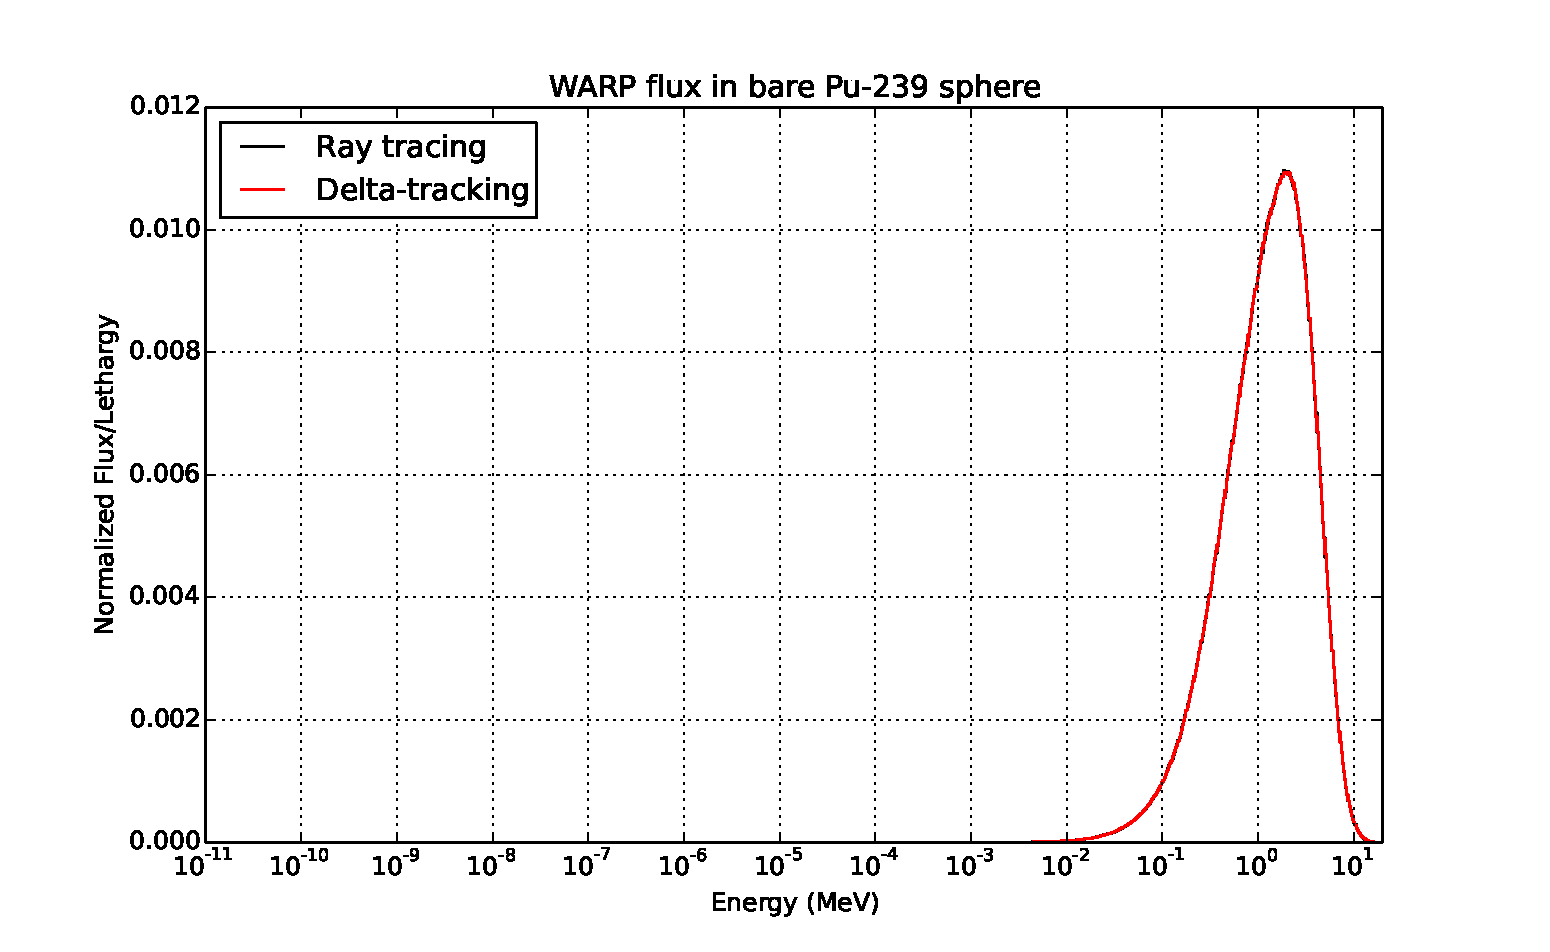
\includegraphics[width=\textwidth]{img/godiva.eps}
\caption{Normalized flux spectra for the Jezebel configuration generated by both versions of WARP.
\label{jezebel}}
\end{figure}

The multiplication factors calculated by each method match within statistical uncertainty and the flux
spectra are nearly (if not actually) identical. The runtimes are comparable for both 
methods. Here, it should not be expected that the delta-tracking method would be considerably different 
compared to the ray tracing algorithm, as the system only contains one cell with one material composed of 
a single isotope.

\subsection{Homogenized block}

The ``homogenized block" test consists of one cube with edges 20 cm in length. The cube is composed of a
homogeneous mixture of 10\% $\ce{^{235}U}$ enriched $\ce{UO_2}$ and water at a 1:1 ratio \cite{warp2015}.
While still a homogeneous case, the homogeneous block is more complex than the Jezebel scenario in that
its single material is composed of multiple isotopes. We are again testing that the delta-tracking
method calculates accurate results, but it is expected that the extra calculations involved in determining
the majorant cross section and the extra OptiX trace needed in the delta-tracking routine will cause an 
increase in runtime. Results for the homogenized block configuration are shown in Table \ref{hom_table} 
and Figure \ref{homfuel}.

\begin{table}[h!]
\centering
\caption{Calculated multiplication factors and runtimes for the homogenized block configuration.}
\label{hom_table}
\begin{tabular}{| c | c | c |}
\hline
\textbf{Method} & $\mathbf{k_{\mathrm{eff}}}$ & \textbf{Runtime} \\
\hline
Ray tracing & $1.213833 \pm 2.9255 \times 10^{-4}$ & 28.14 s \\
Delta-tracking & $1.213983 \pm 2.1413 \times 10^{-4}$ & 30.51 s \\
\hline
\end{tabular}
\end{table}

\begin{figure}[h!]
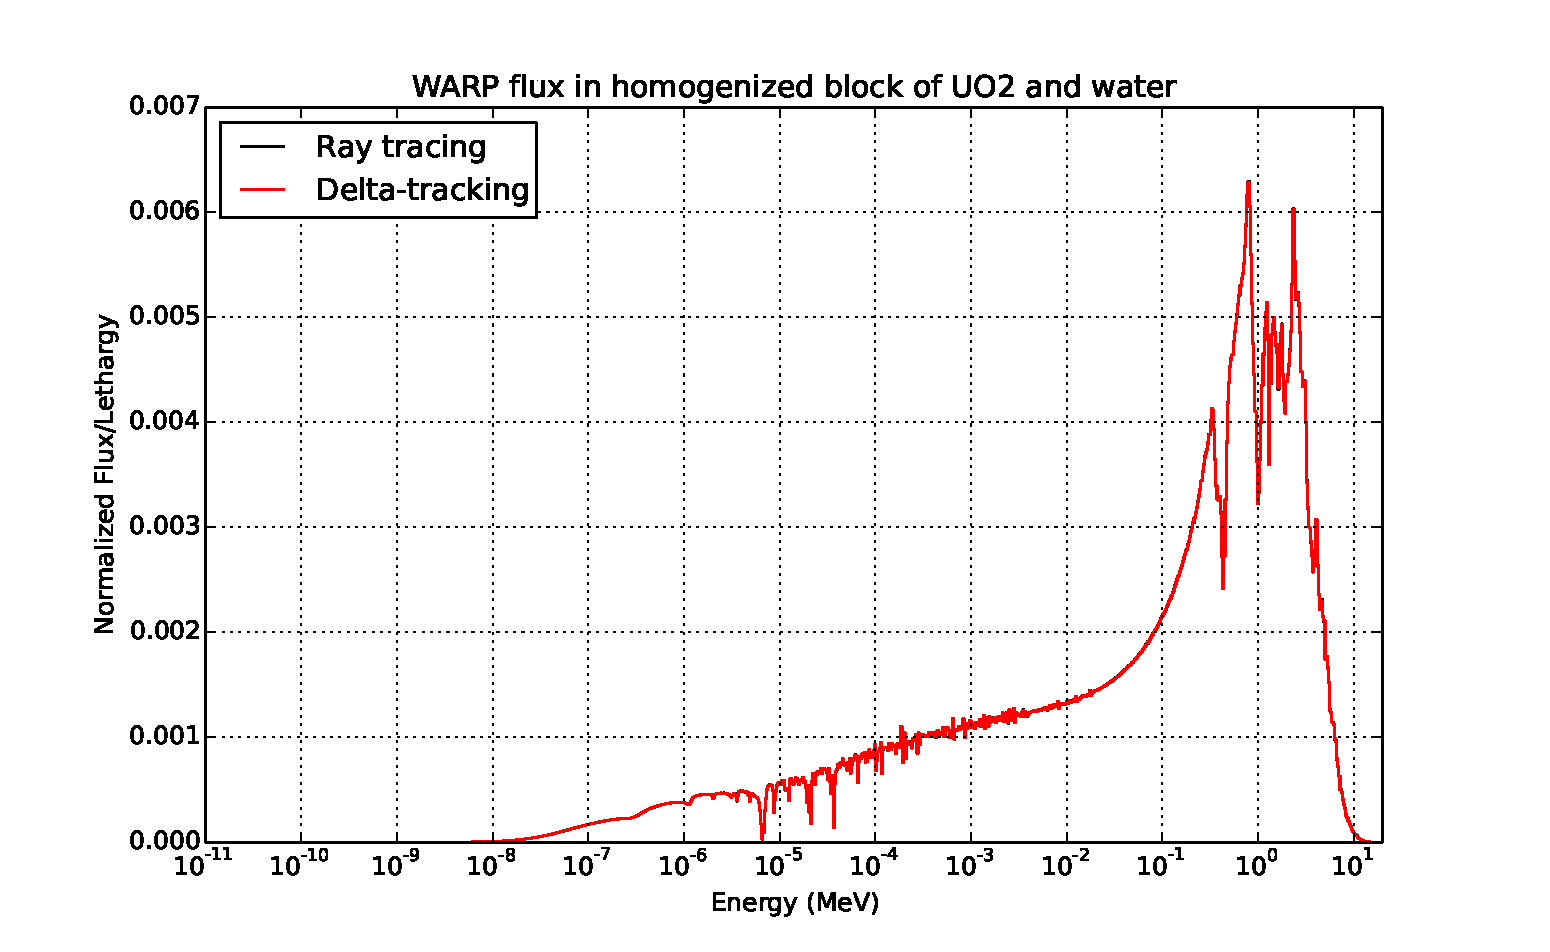
\includegraphics[width=\textwidth]{img/homfuel.eps}
\caption{Normalized flux spectra for the homogenized block configuration generated by both 
versions of WARP. \label{homfuel}}
\end{figure}

Again, the multiplication factor calculated by the delta-tracking version of WARP matches that calculated
by the ray tracing version of WARP (within statistical error). The flux spectra are also consistent with
one another. However, this case shows a greater discrepancy in the runtimes of each of the two methods. 
The version of the code that uses the delta-tracking method is considerably slower, likely because of the
extra calculations required to compute the majorant cross section and the additional OptiX trace required 
in each run.

\section{Heterogeneous systems}
\label{sec:hetero}

For the heterogeneous systems, we are once again testing that the delta-tracking method produces results
that are statistically accurate compared to results calculated using the ray tracing algorithm. However,
for these systems it is expected that the delta-tracking method may be faster than the ray tracing
algorithm. Although additional calculations are incurred in the determination of the majorant cross
section and the additional OptiX trace required for the delta-tracking routine, the time saved in not 
having to stop neutrons at each material boundary may be enough to result in a reduction in runtime with 
the use of the delta-tracking method.

\subsection{Fuel pin cell}

The ``pin cell" test contains a bare $\ce{UO_2}$ cylinder encased in a block of water. The pin has a 
diameter of 1 cm and a length of 40 cm; the dimensions of the surrounding water block are 10 $\times$ 10
$\times$ 50 cm \cite{warp2015}. This test has two materials, each with multiple isotopes, and two cells.
Results can be seen in Table \ref{pin_table} and Figures \ref{pincell-fuel} and \ref{pincell-water}.

\begin{table}[h!]
\centering
\caption{Calculated multiplication factors and runtimes for the pin cell configuration.}
\label{pin_table}
\begin{tabular}{| c | c | c |}
\hline
\textbf{Method} & $\mathbf{k_{\mathrm{eff}}}$ & \textbf{Runtime} \\
\hline
Ray tracing & $3.798339 \times 10^{-1} \pm 6.3999 \times 10^{-4}$ & 3.66683 min \\
Delta-tracking & $3.822616 \times 10^{-1} \pm 4.9758 \times 10^{-4}$ & 3.703 min \\
\hline
\end{tabular}
\end{table}

\begin{figure}[h!]
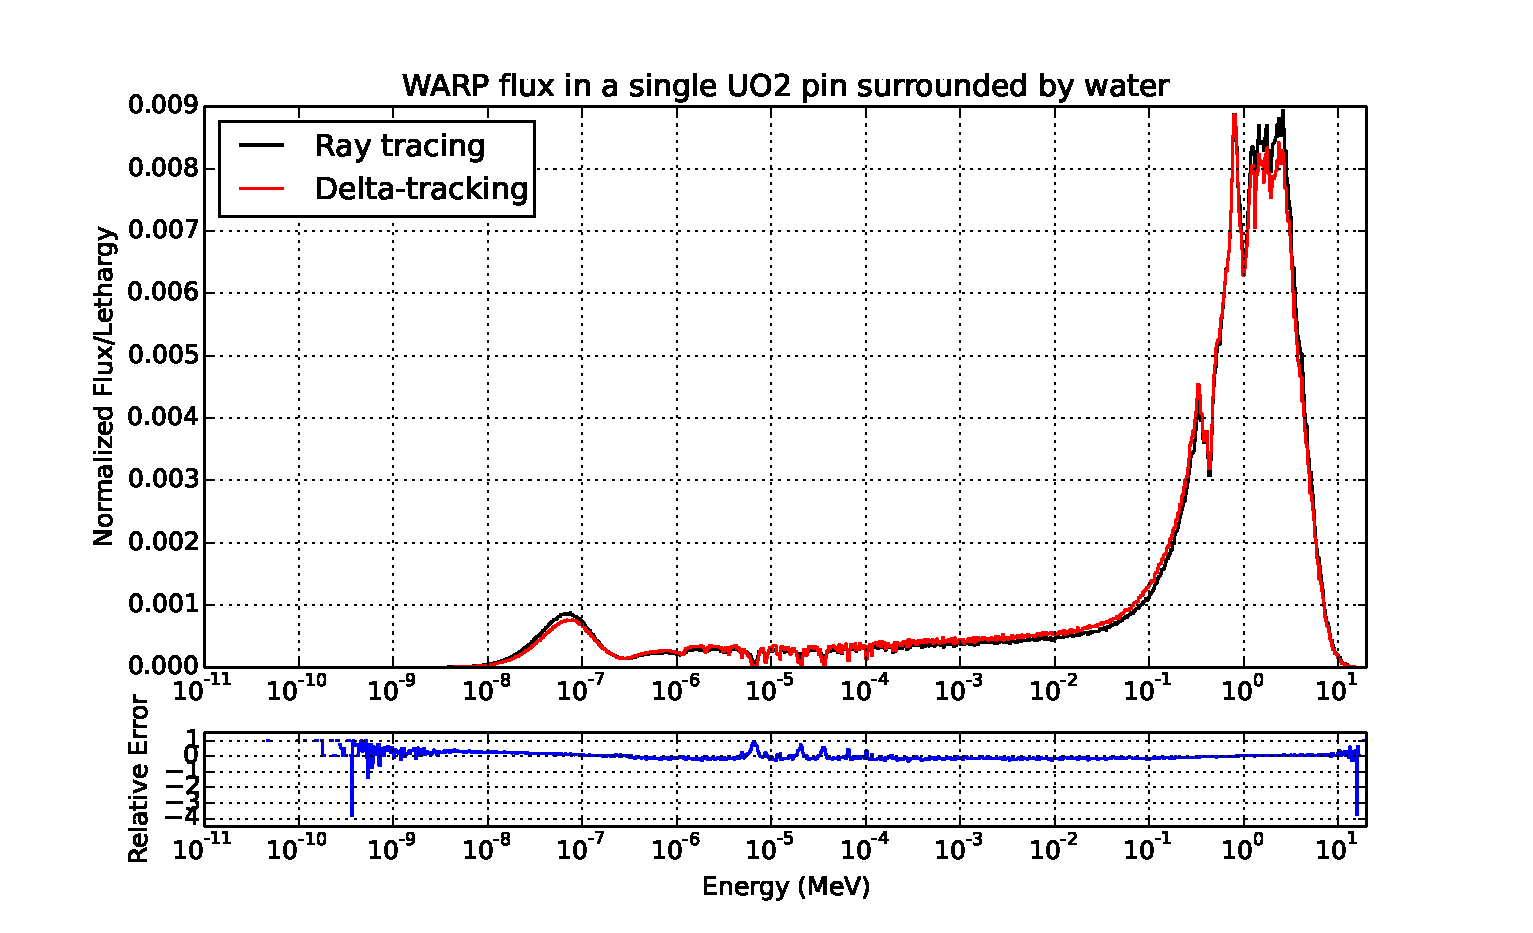
\includegraphics[width=\textwidth]{img/pincell-fuel.eps}
\caption{Normalized flux spectra for the \textbf{$\ce{UO_2}$ cylinder} in the pin cell 
configuration generated by both versions of WARP. \label{pincell-fuel}}
\end{figure}

\begin{figure}[h!]
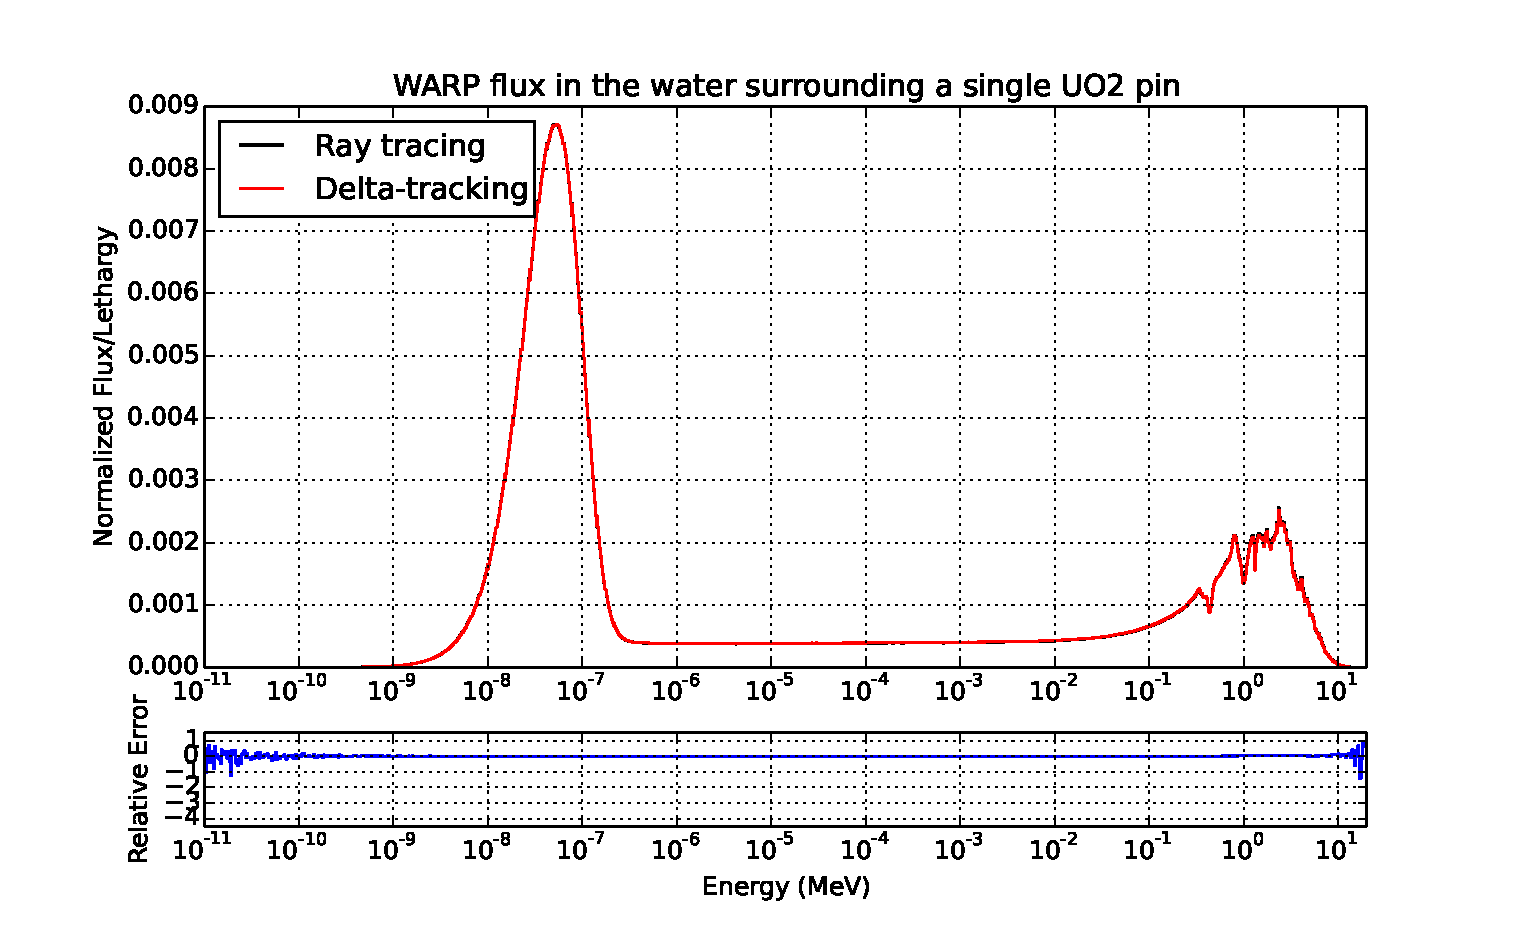
\includegraphics[width=\textwidth]{img/pincell-water.eps}
\caption{Normalized flux spectra for the \textbf{water} block in the pin cell configuration 
generated by both versions of WARP. \label{pincell-water}}
\end{figure}

In this basic, but heterogeneous, configuration, delta-tracking does not accurately calculate the 
multiplication factor for the system. Although the two values look similar, they do not match within
statistical uncertainty. Additionally, large discrepancies are seen in the neutron flux spectra in both
the fuel pin as well as the water surrounding it.

Figure \ref{pincell-fuel} shows that the flux spectrum in the fuel generated by the delta-tracking version
of WARP has slight but noticeable discrepancies compared to the flux spectrum generated by the original 
ray tracing version of the code. The fast and thermal flux are both underestimated, while the epithermal 
flux is overestimated. However, Figure \ref{pincell-water} shows that the flux spectrum in the water 
generated by the delta-tracking version matches the spectrum generated by ray tracing quite well. 

Note that the issues in the calculation of the effective multiplication factor and the normalized flux
spectrum in the fuel of the pin cell align. That is to say, there are more neutrons counted in the fuel in
the case of delta-tracking, and the overestimated value of $k_{\mathrm{eff}}$ also indicates greater 
numbers of neutrons than should actually be present. Since the spectral issue is only seen in the fuel 
(and the value of $k_{\mathrm{eff}}$ applies to the entire system), we may project that the original code 
perhaps has a bug in how fission events are handled. Since no fissions occur in the water, this could be a
potential source of the error seen above.

In this case, delta-tracking is again slower than ray tracing. The extra calculation time likely
comes from the calculation of the majorant at every instance of path length sampling as well as resampling
incurred by the use of the majorant in a system with multiple materials.

\subsection{Fuel pin assembly}

The ``fuel pin assembly" test consists of 631 $\ce{UO_2}$ cylinders arranged in a hexagonal lattice
surrounded by a cube of water with edges of length 84 cm. The material compositions and cylinder 
dimensions are identical to those described above in the pin cell case, but the large number of objects in
this scenario is intended to highlight the effect of introducing many geometric objects into a problem
\cite{warp2015}. Computational results for the fuel pin assembly configuration are shown in Table 
\ref{hex_table} and Figures \ref{assembly-centerpin} and \ref{assembly-water}.

\begin{table}[h!]
\centering
\caption{Calculated multiplication factors and runtimes for the fuel pin assembly configuration.}
\label{hex_table}
\begin{tabular}{| c | c | c |}
\hline
\textbf{Method} & $\mathbf{k_{\mathrm{eff}}}$ & \textbf{Runtime} \\
\hline
Ray tracing & $1.445201 \pm 2.3456 \times 10^{-4}$ & 4.36917 min \\
Delta-tracking & $1.415779 \pm 1.9934 \times 10^{-4}$ & 4.57683 min \\
\hline
\end{tabular}
\end{table}

\begin{figure}[h!]
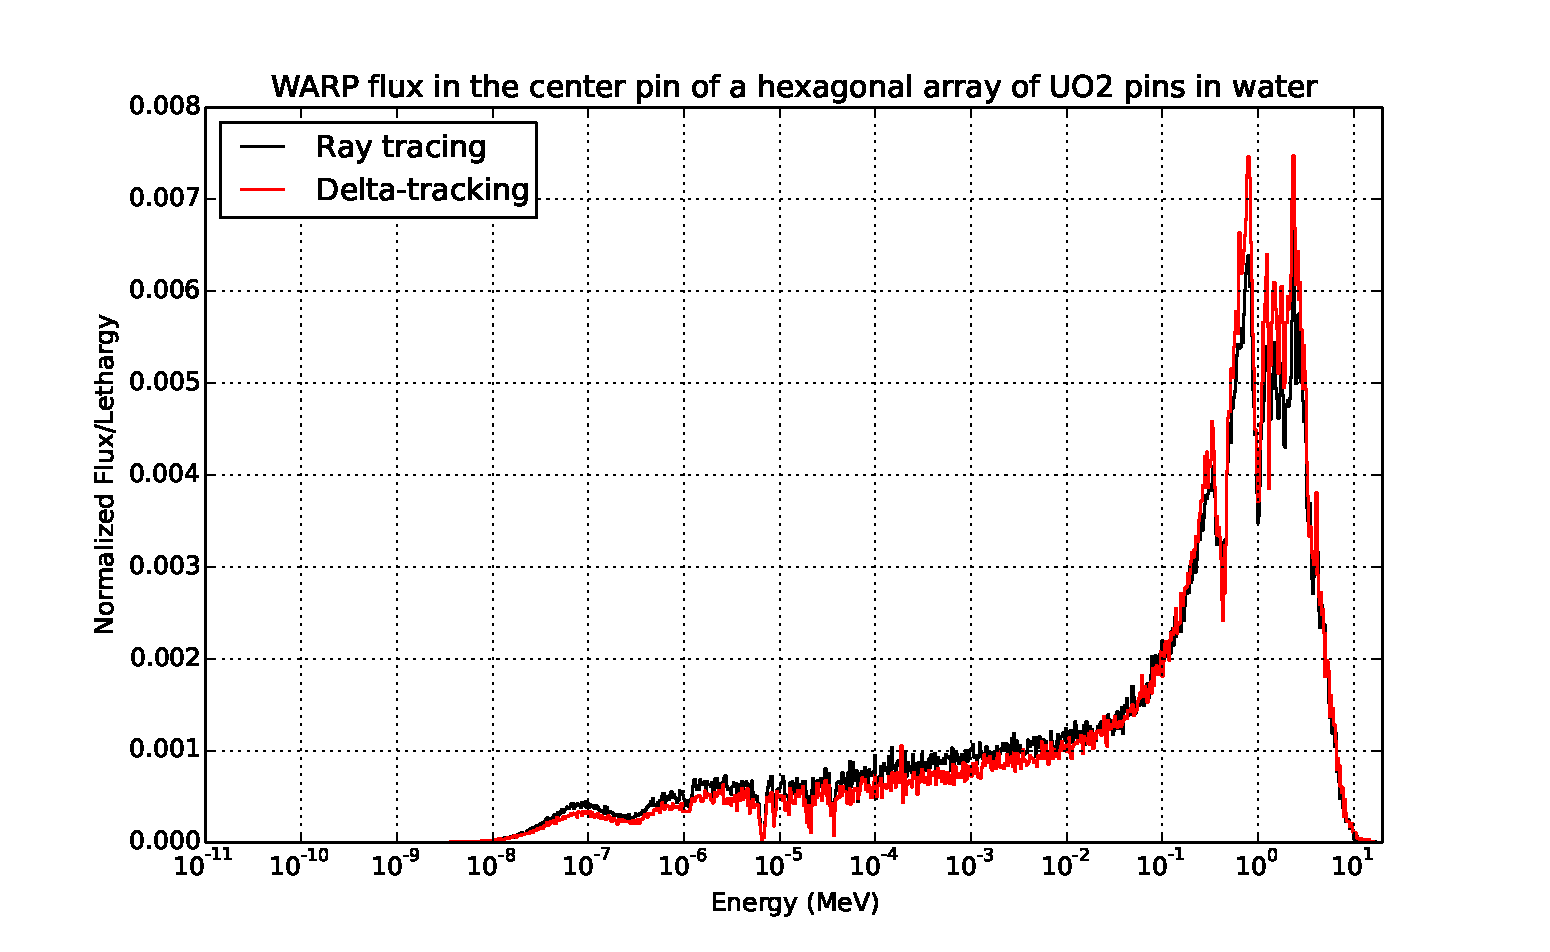
\includegraphics[width=\textwidth]{img/assembly-centerpin.eps}
\caption{Normalized flux spectra for the \textbf{center pin} of a hexagonal array of $\ce{UO_2}$ 
pins in water generated by both versions of WARP. \label{assembly-centerpin}}
\end{figure}

\begin{figure}[h!]
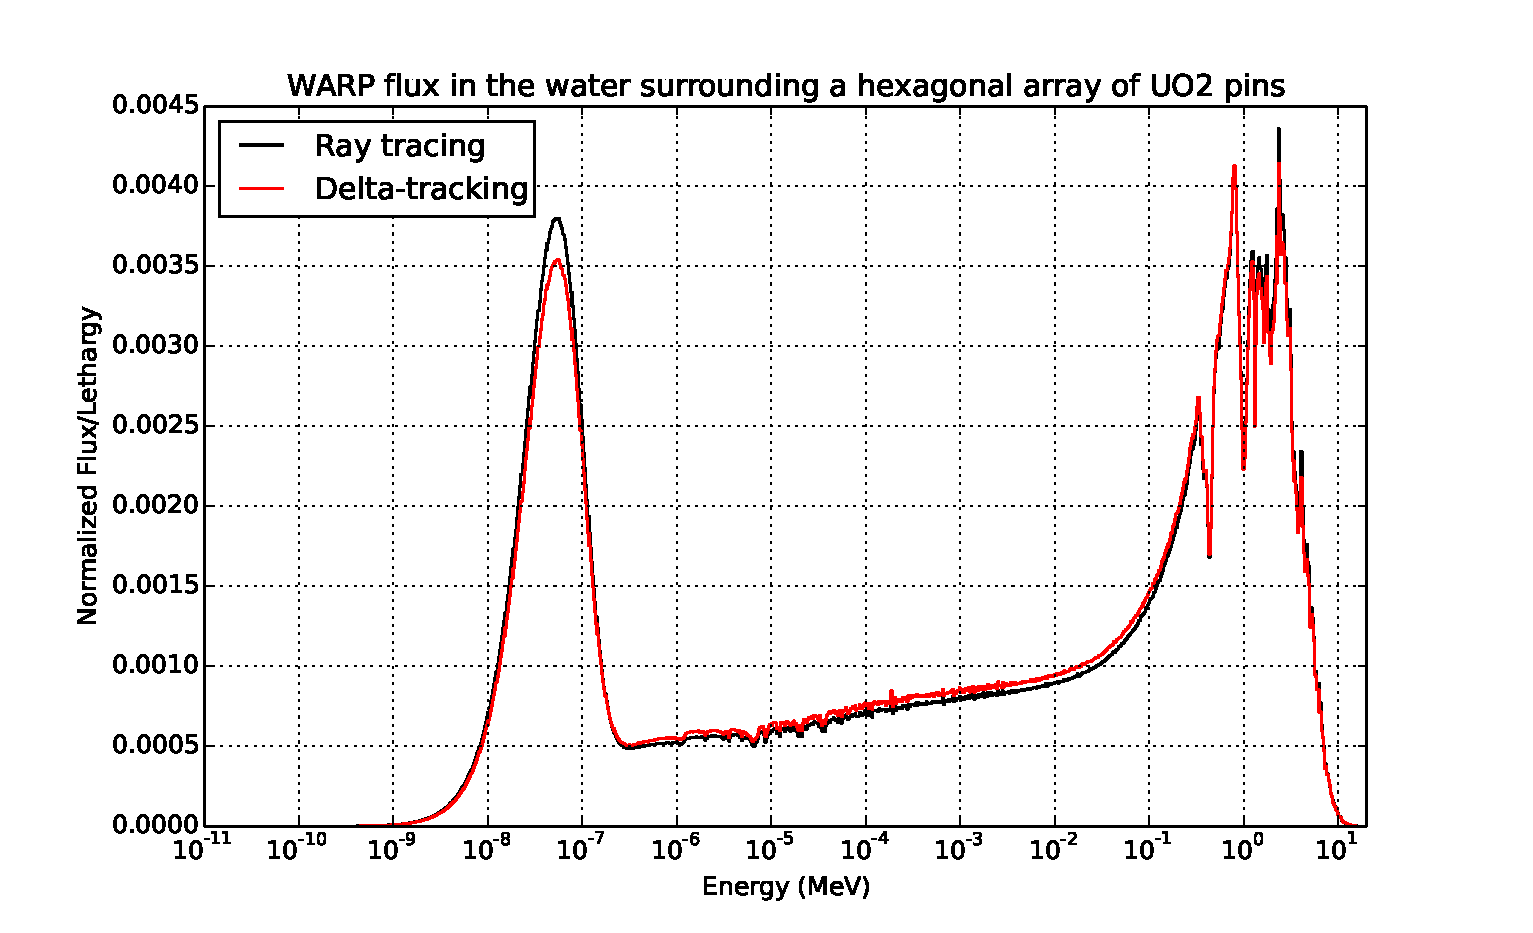
\includegraphics[width=\textwidth]{img/assembly-water.eps}
\caption{Normalized flux spectra for the \textbf{water} surrounding a hexagonal array of 
$\ce{UO_2}$ pins generated by both versions of WARP. \label{assembly-water}}
\end{figure}

The results for the fuel pin assembly simulation suffer from the same geometry issues discussed earlier
in the pin cell simulation results. Using the delta-tracking method causes the neutron multiplication
factor to be grossly underestimated. Spectral issues similar to those in the pin cell configuration are
observed; compared to the spectra generated using ray tracing, too many fast neutrons are in the center 
fuel pin in the assembly and too few thermal neutrons are in the water surrounding the fuel pins.
Given the mismatch in the single pin, this behavior is consistent with expectation.

In addition to these geometrical errors, the delta-tracking method is again slower than the ray tracing
algorithm. Computing the majorant cross section and resampling neutron interactions requires additional
runtime on top of the remainder of the Monte Carlo algorithm.

\section{Experimental homogeneous systems}
\label{sec:exp}

The discrepancies between the two methods in the results of the heterogenous systems prompted the
question of whether the incorrect behavior was caused by the implementation of the delta-tracking method 
or the original code as a whole. The homogeneous systems discussed above were not sufficient to answer 
this question as they contained only one outer boundary.

Taking these notions into consideration, a homogeneous system with artificial boundaries, shown below in 
Figure \ref{jezebel-shells}, was created to test the delta-tracking method against the ray tracing 
method once more. The material and geometry configuration is identical to the Jezebel configuration
described in Table \ref{test_setup} but with an artifical boundary inserted in the sphere. A more
extreme version of this configuration has four artificial boundaries and is shown in Figure 
\ref{jezebel-five}.

The configurations are obviously non-physical; they were contrived explicitly for the purpose of testing
the delta-tracking method in an environment more complex than the basic homogeneous systems in Section
\ref{sec:homog} but less complex than the full-blown heterogeneous configurations in Section 
\ref{sec:hetero}. From the results of these simulations we may infer that if the delta-tracking results
match those calculated with ray tracing, the issues observed in Section \ref{sec:hetero} are issues with
the code that already existed prior to the introduction of the delta-tracking method. If the results are
inconsistent, however, we may conclude that there is an error in the implementation of the delta-tracking
method.

\begin{figure}[h!]
\centering
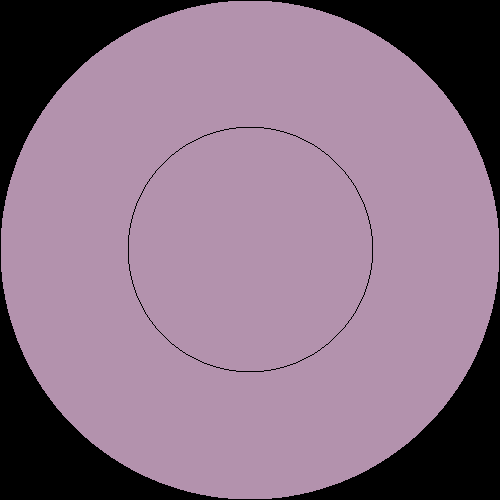
\includegraphics[width=0.5\textwidth]{img/jezebel-shells.png}
\caption{Plot of ``Jezebel" configuration with an inserted artificial boundary. \label{jezebel-shells}}
\end{figure}

\begin{figure}[h!]
\centering
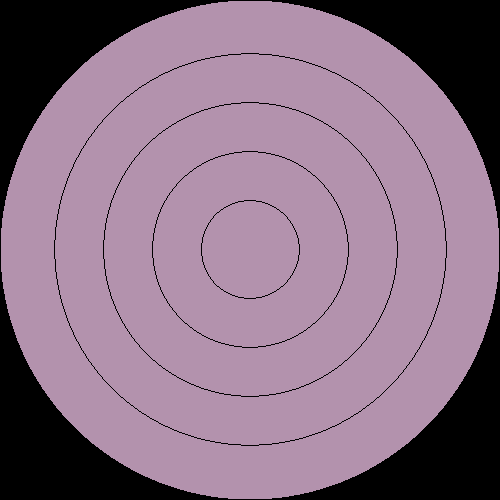
\includegraphics[width=0.5\textwidth]{img/jezebel-shells-five.png}
\caption{Plot of ``Jezebel" configuration with four artificial boundaries. \label{jezebel-five}}
\end{figure}

Results of simulations of the two experimental homogeneous systems follow in Tables 
\ref{jezebel_shells_table} and \ref{jezebel_five_table}. The results show that in each case, the
effective multiplication factor calculated using the delta-tracking method corresponds to that calculated
using the ray tracing method (within statistical error). It should be noted that the ray tracing method
referred to here is not the algorithm discussed in Section \ref{sec:rt} but the algorithm discussed in
Appendix \ref{app:A}. In testing these experimental homogeneous configurations, a major error was found
in the original ray tracing algorithm and it was replaced with a more correct method.

\begin{table}[h!]
\centering
\caption{Calculated multiplication factors and runtimes for the Jezebel configuration with one 
artificial boundary.}
\label{jezebel_shells_table}
\begin{tabular}{| c | c | c |}
\hline
\textbf{Method} & $\mathbf{k_{\mathrm{eff}}}$ & \textbf{Runtime} \\
\hline
Ray tracing* & $1.027356 \pm 3.4527 \times 10^{-4}$ & 20.29 s \\
Delta-tracking & $1.027218 \pm 2.7643 \times 10^{-4}$ & 23.79 s \\
\hline
\end{tabular}
\end{table}

\begin{table}[h!]
\centering
\caption{Calculated multiplication factors and runtimes for the Jezebel configuration with four 
artificial boundaries.}
\label{jezebel_five_table}
\begin{tabular}{| c | c | c |}
\hline
\textbf{Method} & $\mathbf{k_{\mathrm{eff}}}$ & \textbf{Runtime} \\
\hline
Ray tracing* & $1.027238 \pm 2.7643 \times 10^{-4}$ & 24.27 s \\
Delta-tracking & $1.027425 \pm 2.7085 \times 10^{-4}$ & 24.06 s \\
\hline
\end{tabular}
\end{table}

Again, the runtimes of the two methods are comparable, with the delta-tracking method actually outpacing
the new ray tracing algorithm for the case of the Jezebel configuration with four artificial boundaries.
Because the delta-tracking method is consistent with ray tracing for the cases of configurations with a
single material and multiple cells, we may infer that the issues seen in Section \ref{sec:hetero} are due
to exacerbation of preexisting bug(s) in the code by the delta-tracking method. As a result, one cannot
determine whether or not delta-tracking is a viable neutron tracking routine for good performance on GPUs.
However, the performance of the routine observed in the experimental homogeneous cases above indicates the
potential of the delta-tracking method on GPUs.
